\documentclass{article}

\usepackage[backend=biber,sorting=none]{biblatex}
\usepackage{url}
\usepackage{graphicx}
\usepackage{subcaption}
\usepackage{adjustbox}
\usepackage[bottom]{footmisc}
\usepackage{datetime}
\newdate{date}{08}{08}{2023}
\date{\displaydate{date}}
\addbibresource{references.bib}

\title{CS742 Assignment One}
\author{Florian Suess}

\begin{document}

\maketitle
We answer the following questions within the context of the given paper "Workload Characterization of a Large Systems Conference Web Server" by Mahanti et al.\cite{mahanti2009}.
\section*{(Q1) Measurement approaches}
We shall adhere strictly to the definition provided by RFC7799\cite{rfc7799}. There are two measurement mechanisms used;

\begin{itemize}
				\item Analysis of the structured server logs produced during the period of the study.
				\item Google Analytics (GA) data that is a web analytics service that uses a "page tagging" approach to collect data about website traffic and user interactions.
\end{itemize}

Not controversial; \textbf{the analysis of structured server logs provide a form of passive measurement} due to the assumed, async (likely buffer flushing) local writing of these logs into files, an event that itself does not at all influence server side network IO.

In class, GA was introduced as an active measurement approach on the basis that the implementation details of this mechanism necessarily impact the edge network portion to transmit data to the GA analysis server. However the network packets themselves, and their influence on the network itself are not the basis for measurement. Instead the metrics used for measurement are already captured pre-launch by the paging mechanism, \textbf{hence GA is also a form of passive measurement}. Suppose this argument is not accepted, that would imply that analysing modern server logs would be considered active as most production systems that require log analysis emit logs off of systems onto persistence storage systems, or text-search optimised platforms such as Kibana or OpenSearch. This emission would, similar to GA, introduce edge network traffic.

\section*{(Q2-3) Measurement vantage points}
\subsection*{(Q2) Type of measurement vantage used}
Given the client-side and server-side source of both measurement mechanisms, we can confidently narrow say these measurement vantage points to network edge as opposed to core.

\subsection*{(Q3) Quantity of viewpoints considered}
The server-side logs provide a single viewpoint, whilst the client-side measurements provide a very large quantity of viewpoints as most clients (with JS execution enabled) visiting will collect their own metrics.

\section*{(Q4) Hardware and software tools used}
For metric collection and aggregate metric analysis; there were no physical measurement devices deployed. The logs can be assumed to be a natural bi-product of the server running that we collected after the study for analysis using some sort of programming language and GA is by definition a software as a service offering.
 

\section*{(Q5) Online and/or offline analyses performed}
For all practical purposes, metrics collected were analysed post the server study period which as per lecture posits the "analysis" done falls into the "offline" criteria. This is at mercy to the implementation details of GA however, perhaps there is real-time analysis done on the client side that aggregates results before shipping them off to GA analytics platform, in which case implies a component of "online" analytics.

\section*{(Q6) Attributing metrics to Active and/or Passive measurements}
The result in Q1 moots this question, as we have asserted that both measurement mechanisms used are considered "passive". Implies that all metrics materialised in this study are a result of "passive" measurements.

\section*{(Q7) Modern approach on workload characterization of internet servers}
\begin{itemize}
				\item client-side measurement, assuming the server is at least reachable.
				\item traffic interception methods, as described in lectures.
				\item permission to access the server for logs
\end{itemize}

\newpage
The following sections provide an approach for the analysis of the \texttt{ls -lR} output file. Full set of scripts available are provided.
\section*{Notes on querying \texttt{ls} output methodology}
The following questions given to me suggest the use of a queryable interface can be advantageous, whilst the plotting requirements to me speak intervention needed by something like \texttt{python}'s \texttt{matplotlib} hence a well interoperable store is favourable. We are dealing with a very small amount of data.  With all of this in mind; we can sufficiently depend on something lightweight like a local \texttt{sqlite} instance. Hence we will;

\begin{enumerate}
				\item Process the \texttt{ls} output into a \texttt{csv} format.
				\item Spin up a \texttt{sqlite} instance and load a simple table with this \texttt{csv}.
				\item Perform migrations if nessecary (such as extracting the file extension).
\end{enumerate}

One can utilize \texttt{awk}\footnote{Would in practice probably use something more elaborate like a \texttt{go} script.} to parse this output into a \texttt{csv} with the following two pattern match blocks.
\begin{small}
\begin{verbatim}
/:$/{gsub(":",""); dir=$0; next}
$9{print $9 "," dir "," $5 "," $6 " " $7 "," $8}
\end{verbatim}
\end{small}

First one \texttt{/:\$/} matches any lines with a colon and updates the \texttt{dir} variable for interpolation in the next block. Second match ensures there's 9 string parts in the line, if so, converts the ls output line into a csv line of shape; "file name", "dir", "bytes", "day month", "year".

This somewhat awkward looking choice is made because of some lazy date stamps given;
\begin{small}
\begin{verbatim}
-rw-------   1 carey    www2007       0 Aug 28 13:24 allfiles.out
\end{verbatim}
\end{small}
Without a year provided, we need to infer it. We shall assume that year represents 2007 (end of study period). We write a simple \texttt{go} script that looks for a colon in that field, if so, replace it with 2007. We then combine the "day month" and fixed "year" and parse the date into a unix time stamp\footnote{\texttt{sqlite} doesn't offer a native date type hence we will use the \texttt{INTEGER} type in combination with the \texttt{date} function for readability}.

In our \texttt{sqlite} you can bulk upload via $\texttt{.mode csv}$ specifying the seperator as a comma into the following table;

\begin{small}
\begin{verbatim}
CREATE TABLE files (
    file_name TEXT,
    directory TEXT,
    bytes INTEGER,
    last_modified INTEGER
);
\end{verbatim}
\end{small}

\section*{Q8}
\subsubsection*{Quantity of different files}
\begin{small}
\begin{verbatim}
sqlite> SELECT COUNT(*) FROM files;                                 
6062
\end{verbatim}
\end{small}

\subsubsection*{Aggregate sum of file bytes}
\begin{small}
\begin{verbatim}
sqlite> SELECT SUM(size_in_bytes) from files;
1107569732
\end{verbatim}
\end{small}
\textit{Which comes to about 1.107GB.}

\section*{Q9}
\subsubsection*{Largest file on site}
\begin{small}
\begin{verbatim}
sqlite> SELECT MAX(size_in_bytes) FROM files;
59381544
\end{verbatim}
\end{small}
\textit{Which comes to about 59.382MB.}

\subsubsection*{Number of empty files}
\begin{small}
\begin{verbatim}
sqlite> SELECT COUNT(*) FROM files
WHERE size_in_bytes = 0;
15
\end{verbatim}
\end{small}

\subsubsection*{Smallest non-empty file}
\begin{small}
\begin{verbatim}
sqlite> SELECT MIN(size_in_bytes) FROM files 
WHERE size_in_bytes != 0;
2
\end{verbatim}
\end{small}

\section*{Q10}
\subsection*{Mean file size}
\begin{small}
\begin{verbatim}
sqlite> SELECT AVG(size_in_bytes) FROM files;
182706.98317387
\end{verbatim}
\end{small}
\textit{Which comes to about 182.707KB.}

\subsection*{Standard deviation of file size}
\begin{small}
\begin{verbatim}
sqlite> SELECT 
    SQRT(
        AVG(size_in_bytes*size_in_bytes) - 
        (AVG(size_in_bytes) * AVG(size_in_bytes))
    )
FROM files;
2192180.71338199
\end{verbatim}
\end{small}
\textit{Which comes to about 2.192MB.}

\subsection*{Median file size}
Little more tricky given \texttt{sqlite3}'s limitation of no built-in support for median. Recall;
\begin{small}
\begin{verbatim}
sqlite> SELECT count(*) from files;
6062
\end{verbatim}
\end{small}
Hence the median by definition is the average of the middle two file sizes when ordered.\footnote{We could dynamically calculate the median using a \texttt{CASE} on file count also.}
\begin{small}
\begin{verbatim}
sqlite> WITH sorted AS (
    SELECT size_in_bytes,
           ROW_NUMBER() OVER(ORDER BY size_in_bytes) AS rn,
           (SELECT COUNT(*) FROM files) AS cnt
    FROM files
)

SELECT 
    AVG(size_in_bytes)
FROM sorted
WHERE rn IN (cnt / 2, cnt / 2 + 1);
1471.0
\end{verbatim}
\end{small}
\textit{Which comes to about 1.471KB.}

\subsection*{File size mode (most frequently occurring file size)}
\begin{small}
\begin{verbatim}
sqlite> SELECT size_in_bytes, COUNT(*) AS frequency
FROM files GROUP BY size_in_bytes
ORDER BY frequency DESC, size_in_bytes ASC
LIMIT 1;
4096|102
\end{verbatim}
\end{small}
\textit{4096B sized files occured a whooping 102 times!}

\section*{Notes on the plotting methodology}
\texttt{python} in my eyes is the defacto wizard when it comes to graphing due to well-traversed libraries such as \texttt{matplotlib}. Hence we will use the standard library \texttt{sqlite} module in \texttt{python}. Scripts are here to use.

\section*{Q11 - Plotting file size distribution}
We effectively just handle the full list of bytes via;

\begin{small}
\begin{verbatim}
SELECT size_in_bytes FROM files
\end{verbatim}
\end{small}

\begin{figure}[htbp]
\centering

\begin{minipage}{.5\linewidth}
\centering
\subcaption{Probability density graph}
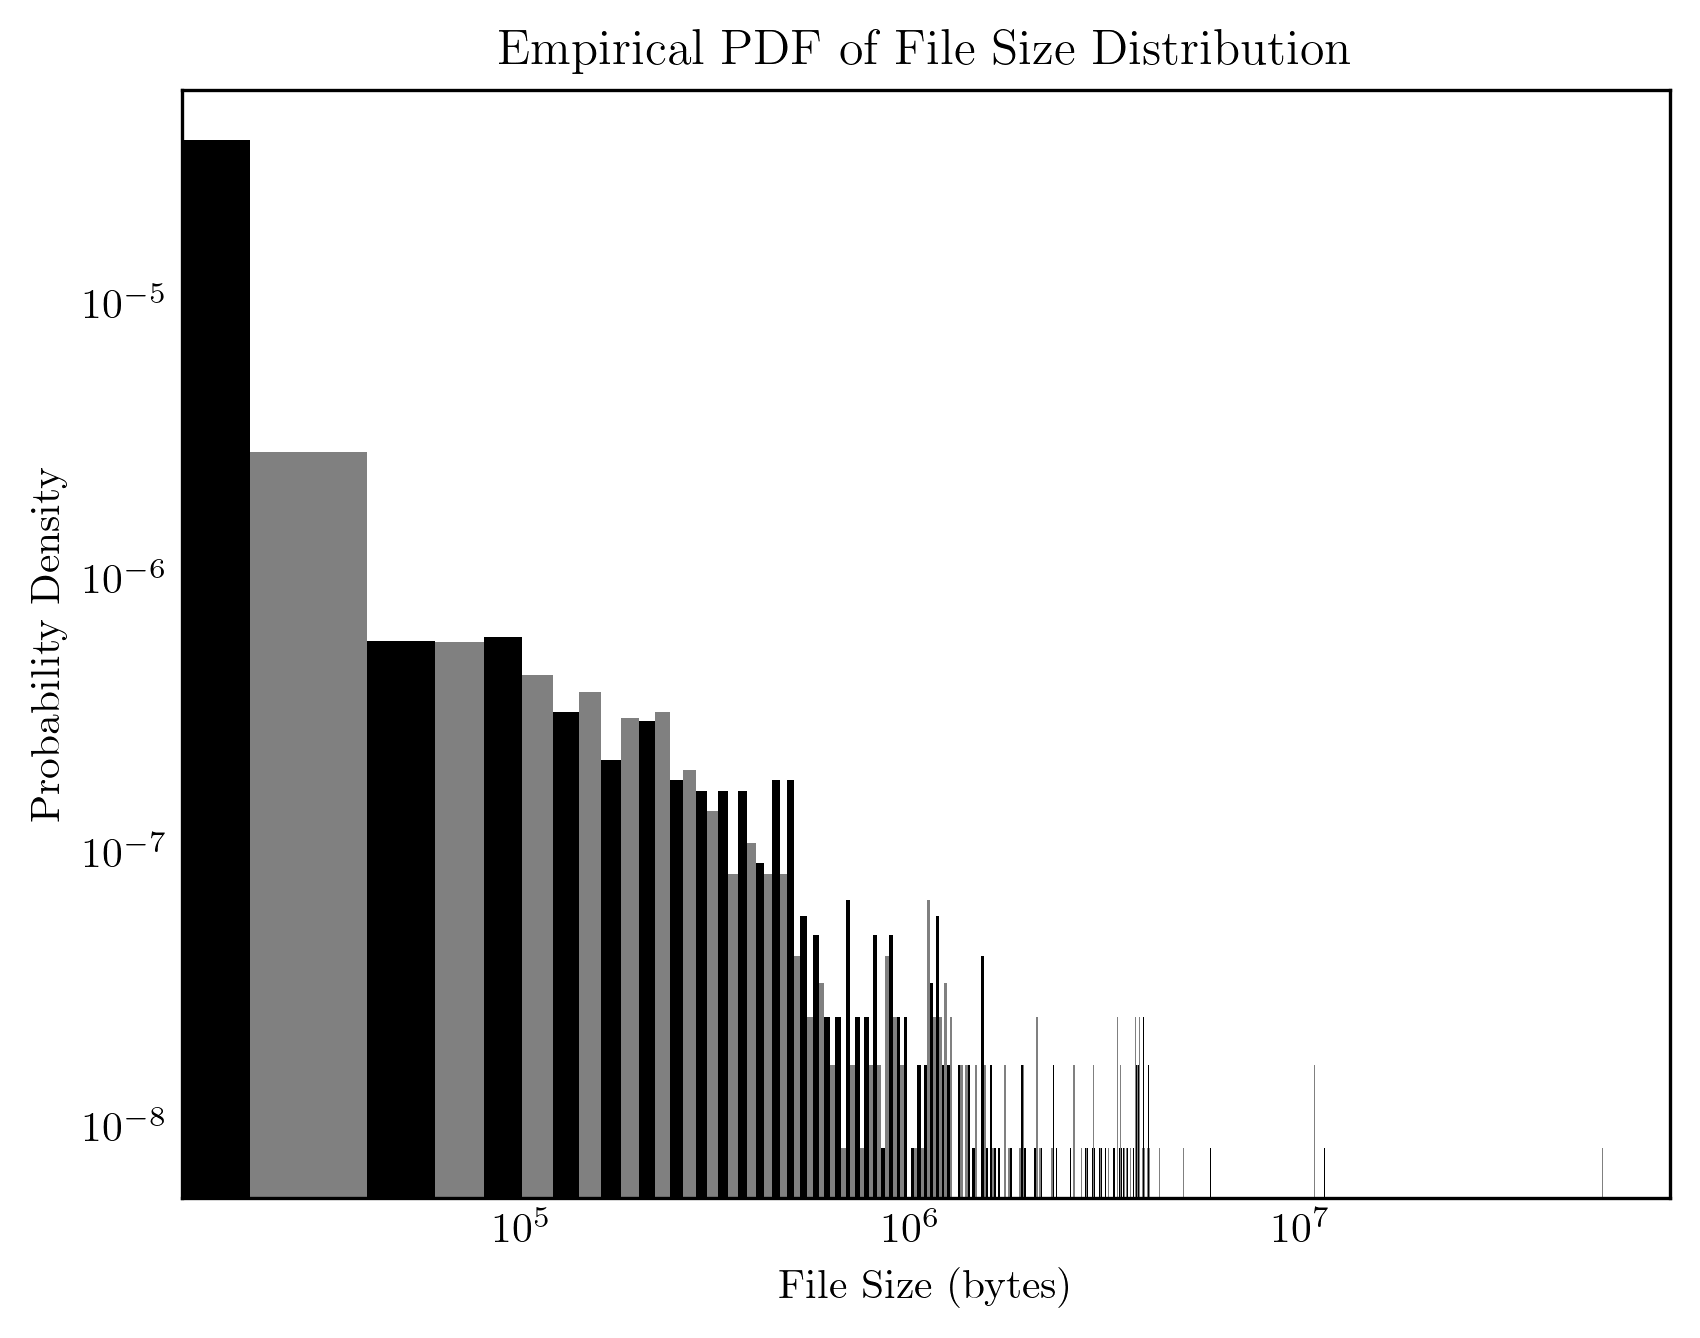
\includegraphics[width=\linewidth]{./images/file_size_pdf.png}
\end{minipage}%
\begin{minipage}{.5\linewidth}
\centering
\subcaption{Cumulative distribution graph}
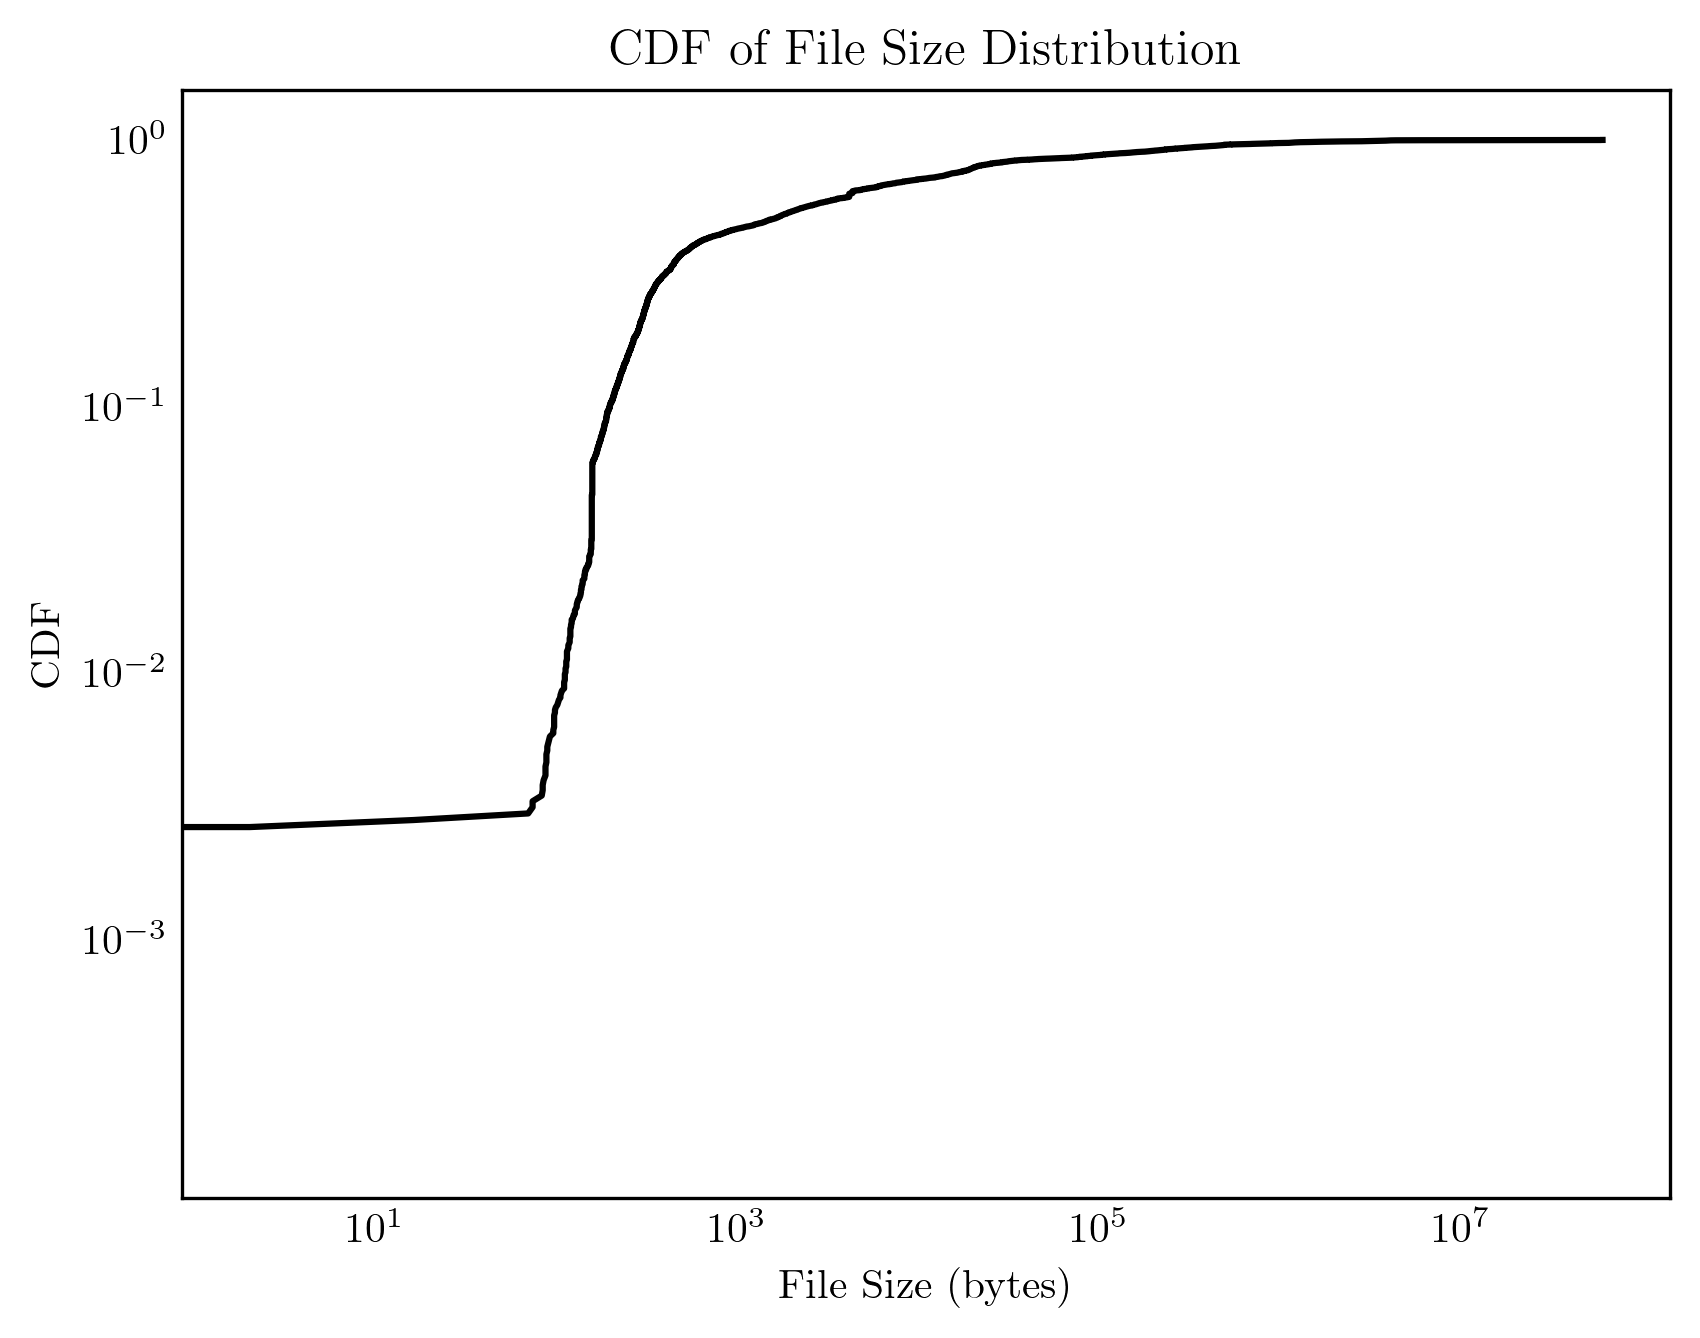
\includegraphics[width=\linewidth]{./images/file_size_cdf.png}
\end{minipage}

\end{figure}

We used a log scale on both of these graphs in order to effectively capture and graph the positively-skewed distribution.

\section*{Q12 - Table of top 10 file types}
We can broadly determine the filetype based on the extension of the filename in our database (defined as the letters after the last dot). Hence we perform the following migration;

\begin{small}
\begin{verbatim}
ALTER TABLE files ADD COLUMN extension TEXT;
\end{verbatim}
\end{small}

\begin{small}
\begin{verbatim}
UPDATE files SET extension = 
REPLACE(file_name,
    RTRIM(file_name, REPLACE(file_name, '.', '')), '');
\end{verbatim}
\end{small}

The latter migration is a common workaround for \texttt{sqlite}'s lack of a last index function\footnote{\url{https://stackoverflow.com/a/38330814}}, but where effectively extracting the substring from the position of the \textbf{last} dot.

\begin{small}
\begin{verbatim}
UPDATE files SET extension = LOWER(extension);
\end{verbatim}
\end{small}

\newpage

\begin{small}
\begin{verbatim}
WITH FileTypeAggregates AS (
    SELECT 
        extension,
        COUNT(*) as file_count,
        SUM(size_in_bytes) as total_bytes
    FROM files
    WHERE extension IS NOT NULL AND extension != ''
    GROUP BY extension
),

Top10 AS (
    SELECT extension, file_count, total_bytes
    FROM FileTypeAggregates
    ORDER BY file_count DESC
    LIMIT 10
),

OtherAggregates AS (
    SELECT 
        'OTHER' AS extension,
        SUM(file_count) as file_count,
        SUM(total_bytes) as total_bytes
    FROM FileTypeAggregates
    WHERE extension NOT IN (SELECT extension FROM Top10)
),

Combined AS (
    SELECT * FROM Top10
    UNION ALL
    SELECT * FROM OtherAggregates
),

TotalAggregates AS (
    SELECT 
        SUM(file_count) as total_files,
        SUM(total_bytes) as total_bytes
    FROM Combined
)

SELECT 
    c.extension AS "Type",
    c.file_count AS "Count",
    printf("%.2f", (c.file_count * 100.0 / ta.total_files))
	        AS "Count Percentage",
    c.total_bytes AS "Total Bytes",
    printf("%.2f", (c.total_bytes * 100.0 / ta.total_bytes))
	        AS "Percentage of Bytes"
FROM Combined c, TotalAggregates ta
ORDER BY CASE WHEN
c.extension = 'OTHER' THEN 1 ELSE 0 END, c.file_count DESC;
\end{verbatim}
\end{small}


This SQL query aggregates file statistics by extension, identifying the top 10 file extensions by count. It provides a breakdown of file counts and their sizes both for these top 10 extensions and for all other extensions combined under "OTHER". The final output displays each file type, its count, its percentage of the total file count, its total bytes, and its percentage of the total bytes, with the "OTHER" category displayed last. Now with \texttt{.headers on} and \texttt{.mode column} we can yield the following table.

\vspace{20pt}
\begin{small}
\begin{verbatim}
Type      Count  Count Percentage  Total Bytes  Percentage of Bytes
--------  -----  ----------------  -----------  -------------------
png       2339   38.58             12220808     1.10               
jpg       905    14.93             337287389    30.45              
gif       656    10.82             3003468      0.27               
php       521    8.59              1947964      0.18               
pdf       362    5.97              545146440    49.22              
txt       249    4.11              32067913     2.90               
svn-base  190    3.13              437769       0.04               
svn-work  190    3.13              29472        0.00               
wmz       133    2.19              81007        0.01               
html      114    1.88              6767416      0.61               
OTHER     403    6.65              168580086    15.22              
\end{verbatim}
\end{small}

\newpage

\section*{Q13 - Plotting file size distribution restricted to \texttt{./papers} and \texttt{./posters}}
In contrast to Q11 when we had to plot PDF functions; we effectively just handle the list of bytes via additional \texttt{WHERE} clauses narrowing down the files to within a certain directory.

\begin{small}
\begin{verbatim}
SELECT size_in_bytes FROM files WHERE directory = "./papers"
\end{verbatim}
\end{small}

And

\begin{small}
\begin{verbatim}
SELECT size_in_bytes FROM files WHERE directory = "./posters"
\end{verbatim}
\end{small}

\begin{figure}[htbp]
\centering

\begin{minipage}{.5\linewidth}
\centering
\subcaption{Papers}
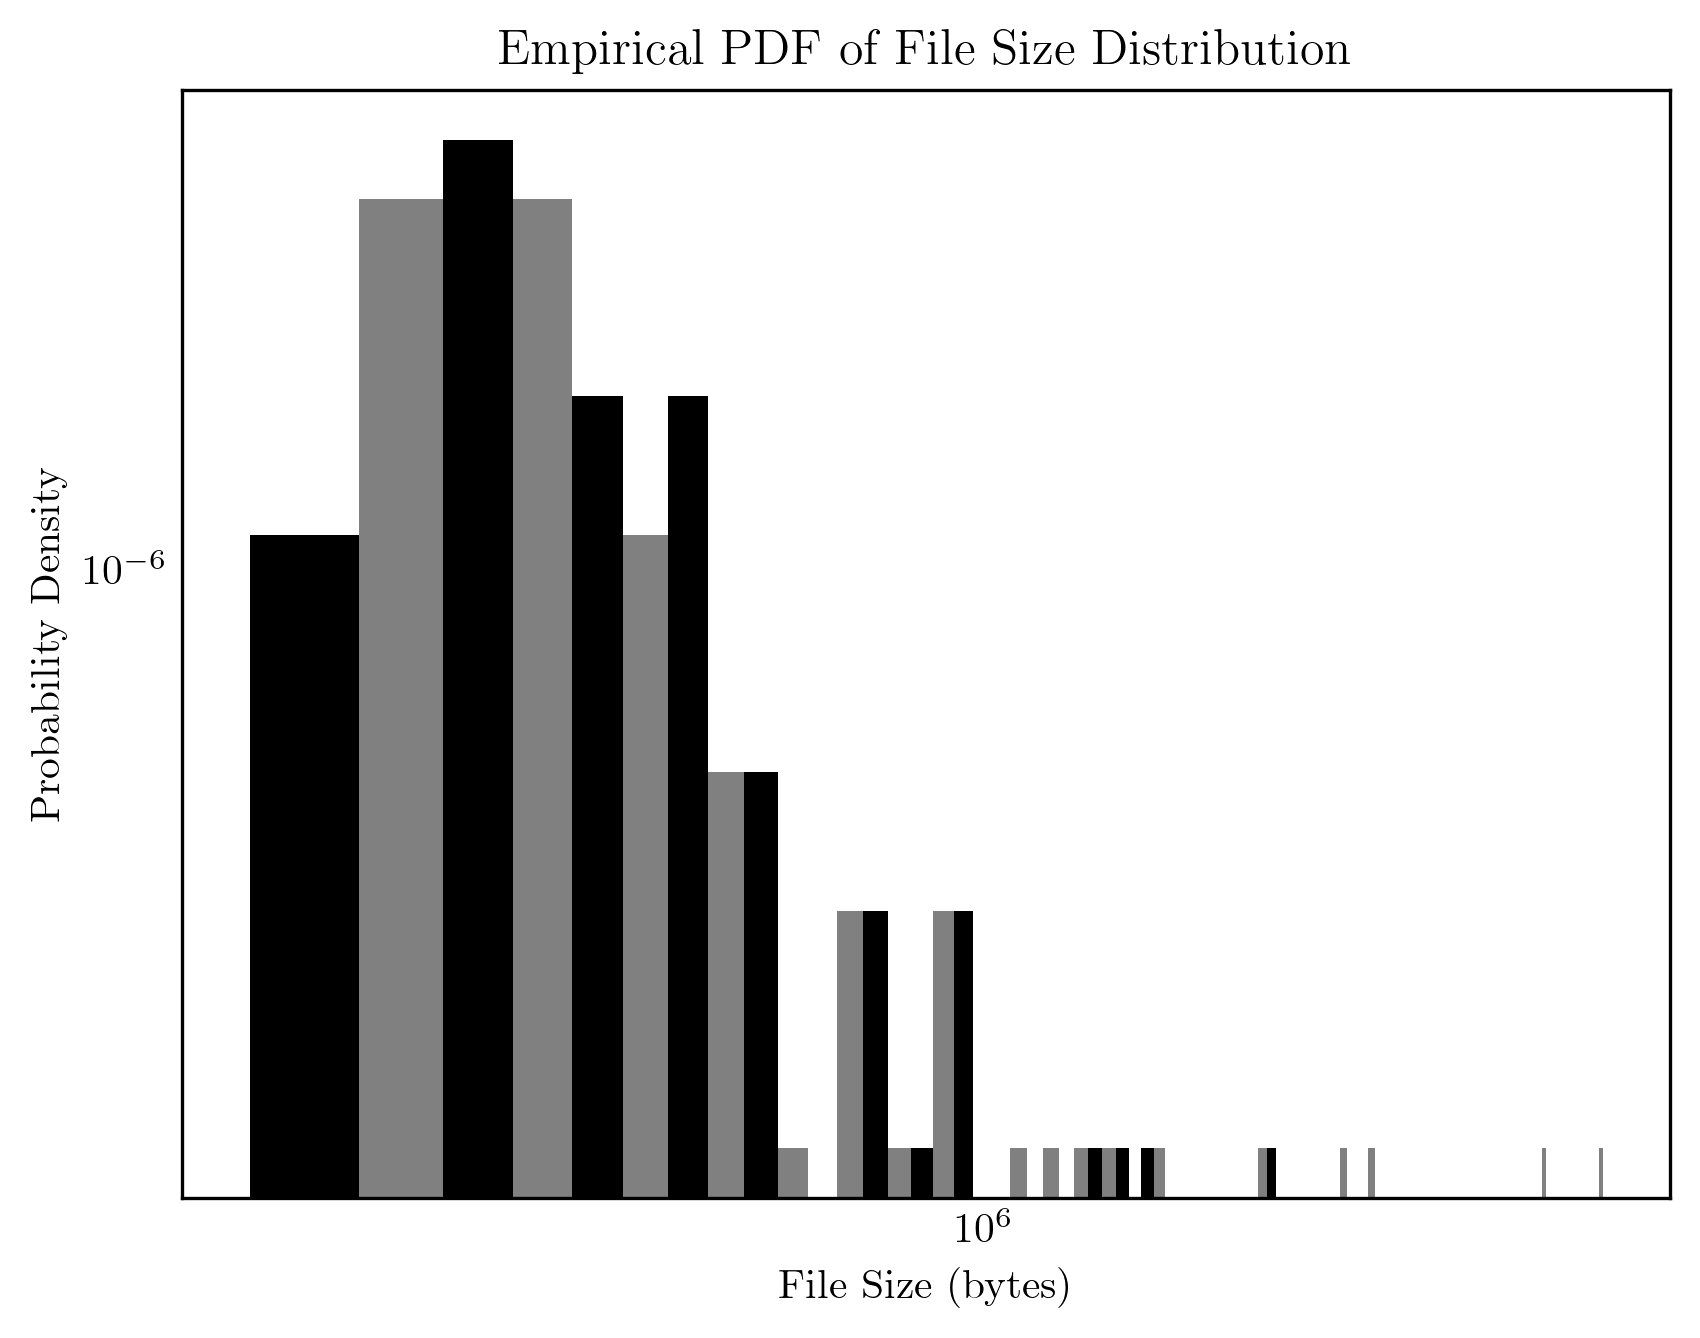
\includegraphics[width=\linewidth]{./images/papers_size_pdf.png}
\end{minipage}%
\begin{minipage}{.5\linewidth}
\centering

\subcaption{Posters}
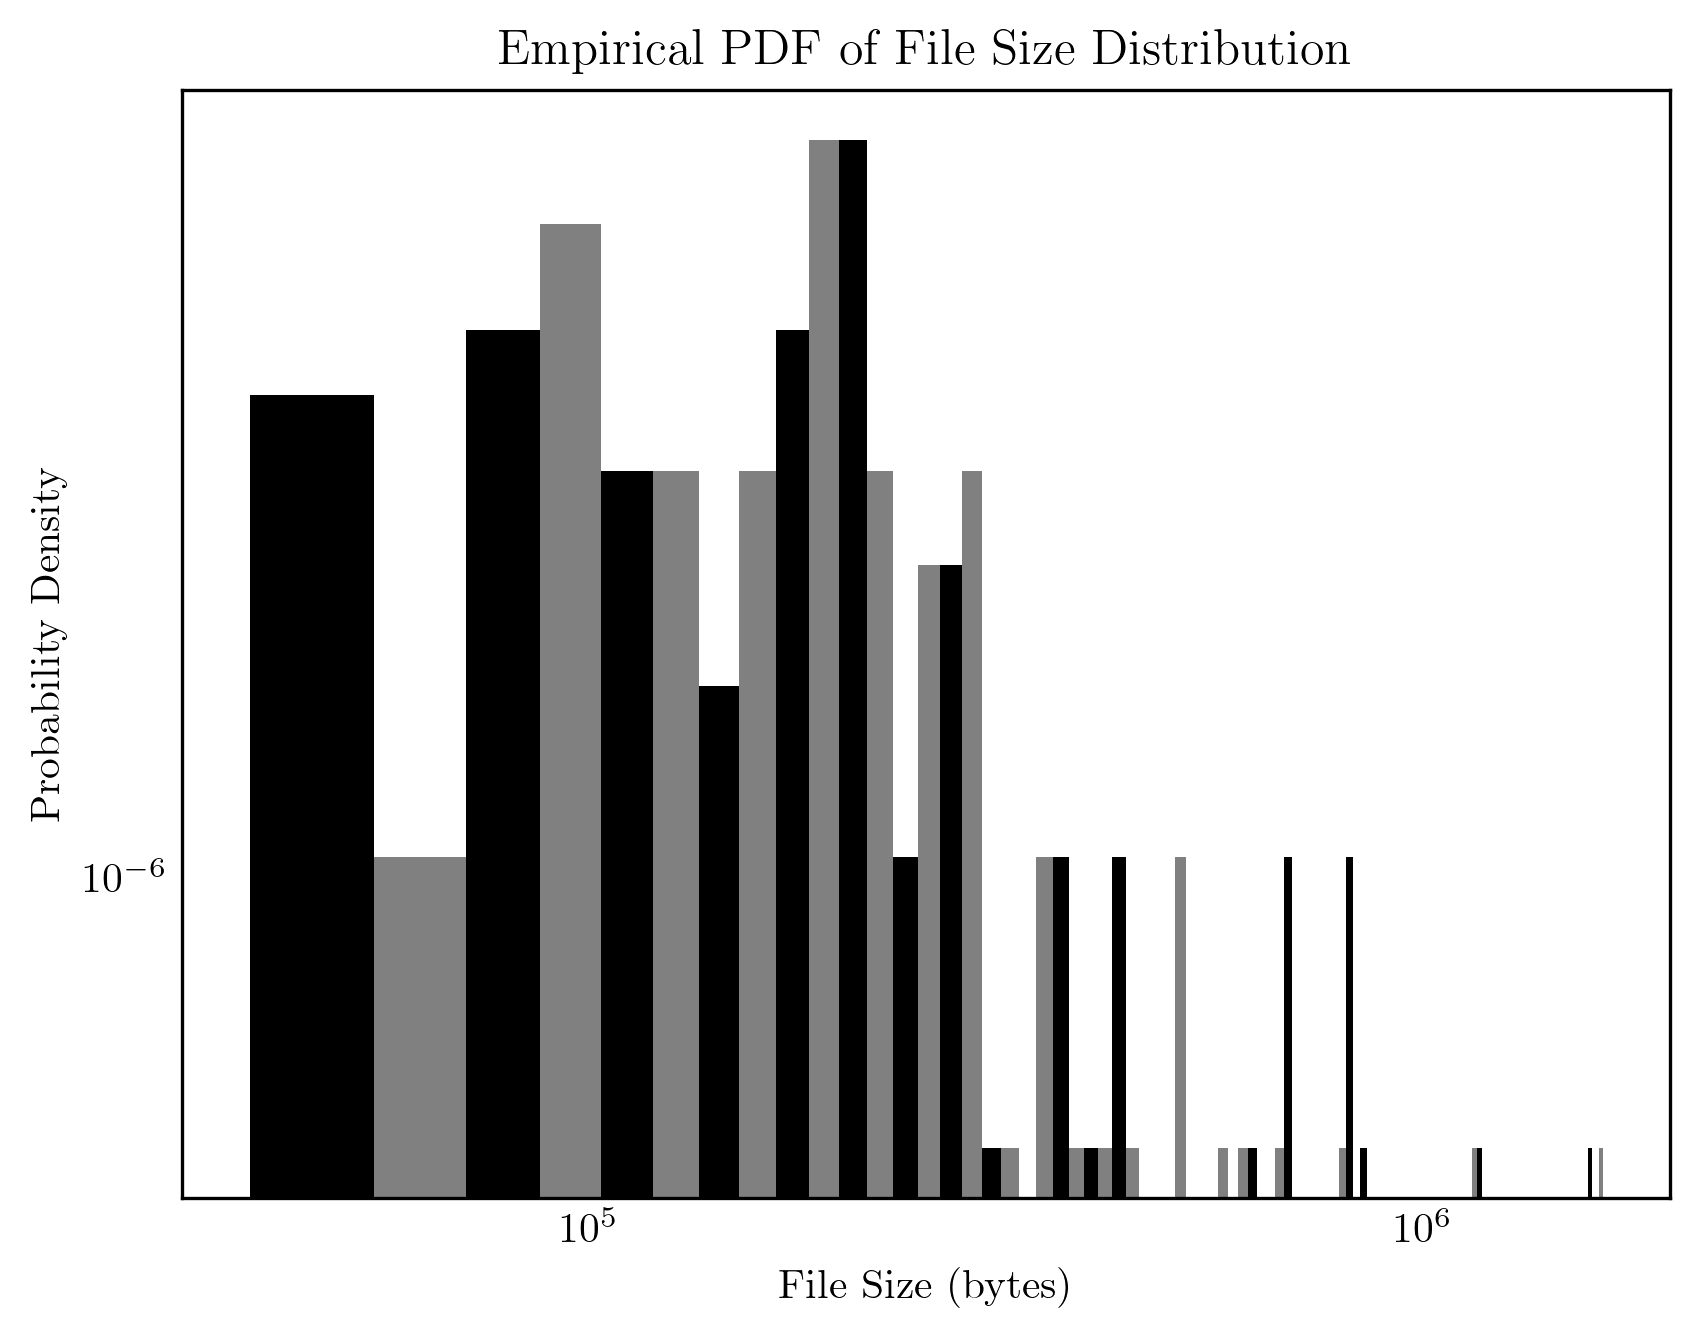
\includegraphics[width=\linewidth]{./images/posters_size_pdf.png}
\end{minipage}

\end{figure}

Both of these distributions are positively-skewed hence the log scale approach applied once again.

\begin{figure}[htbp]
\centering
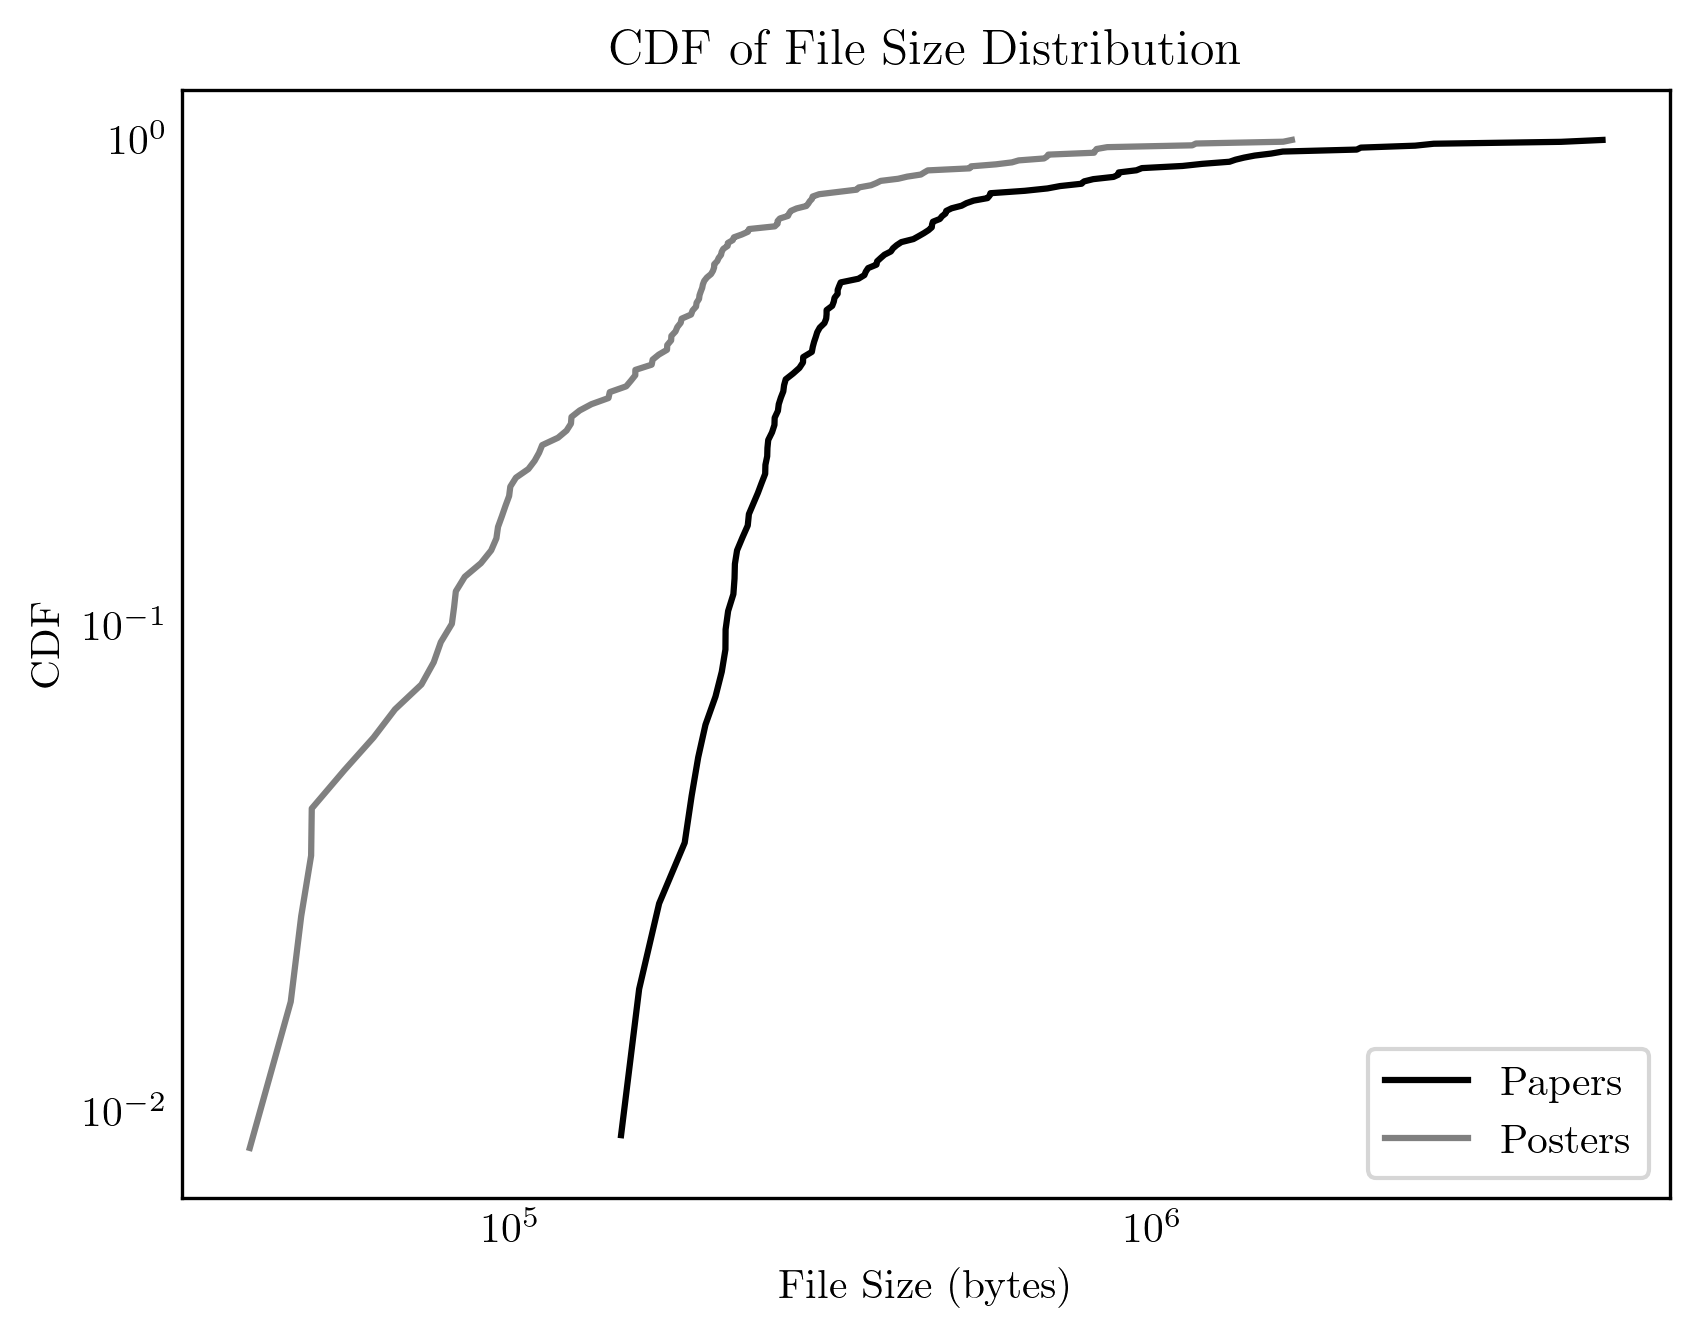
\includegraphics[width=\linewidth]{./images/papers_posters_size_cdf.png}
\end{figure}

\newpage
\section*{Q14 - Analysis of file age}
\subsection*{Hydrating age of each file}
As per original bulk upload, we ensured the date is correctly captured and passed into a \texttt{Unix} \texttt{epoch} timestamp (including the edge case timestamps provided\footnote{parsing the "13:24" included timestamp to be contextualised to the year 2007}) hence we're pre-prepared for this question. Thus when querying for human-readable

\subsection*{The oldest file}
\begin{verbatim}
sqlite> SELECT 
    directory || '/' || file_name,
    date(MIN(last_modified), 'unixepoch')
FROM files;
./images.bak/acmlogo.gif|2006-02-23
\end{verbatim}
\subsection*{The newest file}
\begin{verbatim}
sqlite> SELECT 
    directory || '/' || file_name,
    date(MAX(last_modified), 'unixepoch')                   
FROM files;
./index.php|2008-02-02
\end{verbatim}
\subsection*{Mean file age}
\begin{verbatim}
sqlite> SELECT 
    date(AVG(last_modified), 'unixepoch')
FROM files;
2007-02-03
\end{verbatim}

\subsection*{Median file age}
Recall as per Q10; 

\begin{verbatim}
sqlite> SELECT count(*) from files;
6062
\end{verbatim}

Hence the median by definition is the average of the middle two epoch timestamps when ordered.\footnote{We could dynamically calculate the median using a \texttt{CASE} on file count also.}

\begin{verbatim}
sqlite> WITH sorted AS (
    SELECT last_modified,
           ROW_NUMBER() OVER(ORDER BY last_modified) AS rn
    FROM files
)

SELECT 
    date(AVG(last_modified), 'unixepoch')
FROM sorted
WHERE rn IN (rn / 2, rn / 2 + 1);
2006-02-23
\end{verbatim}

\subsection*{Mode file age}

\begin{verbatim}
sqlite> SELECT
    date(last_modified, 'unixepoch'),
    COUNT(*) AS frequency
FROM files GROUP BY last_modified   
ORDER BY frequency DESC, last_modified ASC
LIMIT 1;
2007-02-19|1159
\end{verbatim}

\newpage

\section*{Q15 - Cumulative distribution function graph of file age}
We effectively just handle the full list of rows returned via;

\begin{small}
\begin{verbatim}
SELECT last_modified FROM files
\end{verbatim}
\end{small}

\begin{figure}[htbp]
\centering
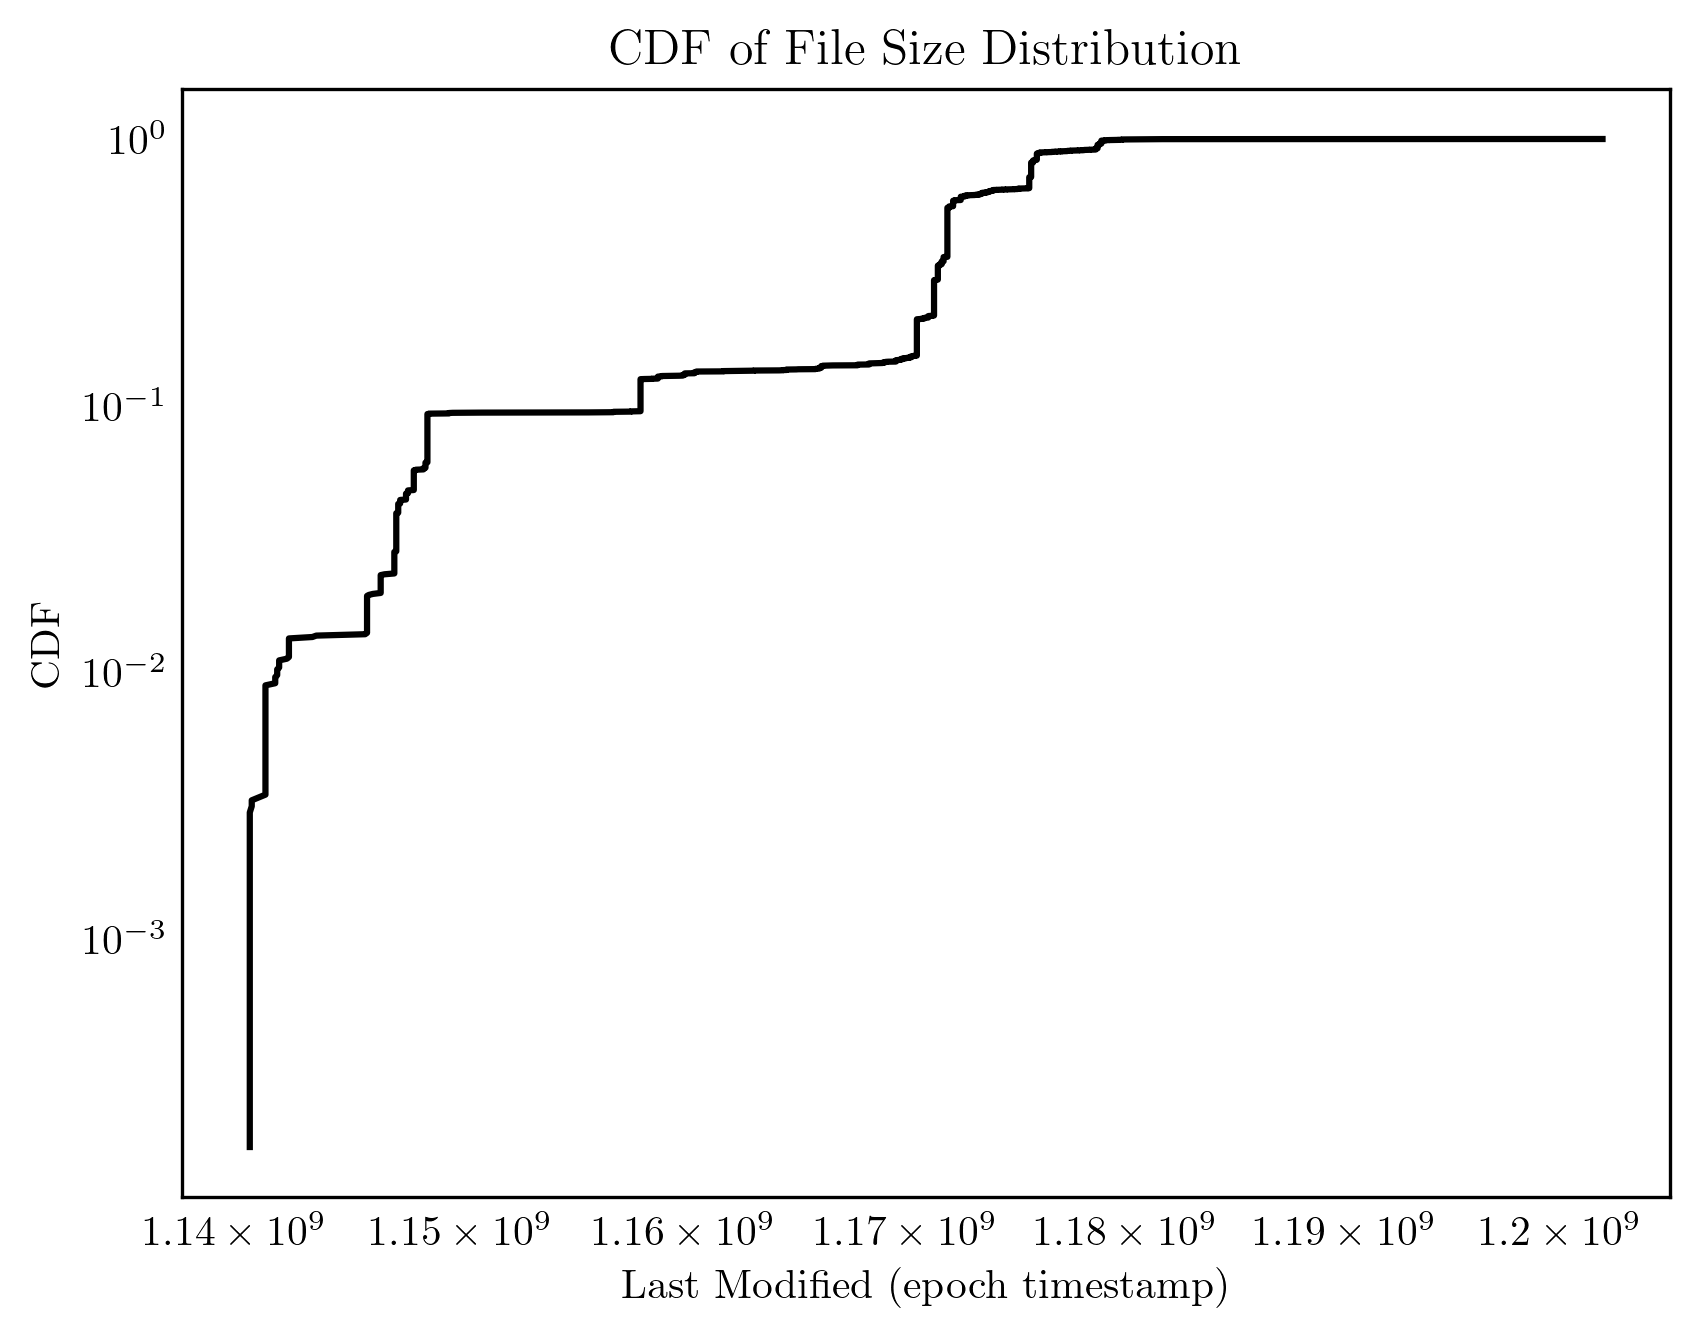
\includegraphics[width=\linewidth]{./images/last_modified_size_cdf.png}
\end{figure}

\newpage
\printbibliography
\end{document}
